
\section{Introduction}

In his \emph{Foundations of Arithmetic}, Frege promises ``never to ask for the meaning
of a word in isolation, but only in the context of a proposition''
\parencite*[xvii]{Frege1980}.
This `context principle' is intuitive: words are frequently polysemous, or assume
different connotations and emphasis within different expressions.
Historically, however, contextuality has been a problem for distributional meaning
representations.
Founded on the distributional hypothesis \parencites{Harris1954}{Firth1957}, both
count-based and predictive models of word meaning\footnote{ This terminological
  distinction is due to \textcite{Baroni2014a}.
} originally
produced a single representation for each word in the model's vocabulary.
One of these \emph{static} representations must, therefore, encode all of a word's
senses and connotations, which is an obstacle to its use in modelling context-dependent
phenomena.

Prior to the widespread availability of pre-trained word embeddings
\parencites[e.g.,][]{Mikolov2013}{Pennington2014}, this problem was generally addressed
by one of two approaches: firstly, by producing a representation for each sense of a
target word and disambiguating between them in the given context (\emph{word-sense
  disambiguation}); or secondly, by composing the representation of the target word with
the representations of the words in its context (\emph{contextualisation}).
These approaches have been largely overshadowed by the advent of model architectures
that take sequences as inputs and naturally produce \emph{contextual} representations
of the items in the sequence, such as Transformers \parencite{Vaswani2017}.

To my knowledge, however, there has been scant direct comparison of the performance of
these contextual representations with the application of prior methods of
contextualisation to static representations.
SemEval-2020 Task 3, ``Graded Word Similarity in Context''
\parencite{Armendariz2020a}, presents an opportunity to make such a comparison.
Briefly, the task is to predict the continuously-valued human judgment of similarity of
the same pair of words in two different contexts (Section~\ref{task-definition}).
I elected to focus on the first subtask, which is to predict the \emph{change} in
similarity, rather than the absolute similarity in each context.
Specifically, I evaluated the results obtained by computing the cosine similarity
between static and contextual representations, and the additive composition of these
representations within a fixed-size context window.

\section{Task definition}
\label{task-definition}

The CoSimLex dataset \parencite{Armendariz2020}, which served to evaluate the task
submissions, extends the SimLex-999 dataset \parencite{Hill2015} to include multiple
contexts for each pair of words.

\section{Related work}

Additive composition \parencites[e.g.][]{Kintsch2001}{Mitchell2008}{Mikolov2013a}.
Analysis of the effect of window size on static embeddings.
Analysis of contextual embeddings.

\section{Methodology}

\begin{figure}
  \centering
  \captionsetup{justification=centering}
  \newcommand{\period}{.}
  \newcommand*{\orawidest}{accept}
  \newcommand*{\oratallest}{\#\#}
  \newlength{\orawidth}
  \settowidth{\orawidth}{\orawidest}
  \newcommand*{\ora}[1]{\overrightarrow{#1\vphantom{\oratallest}}}
  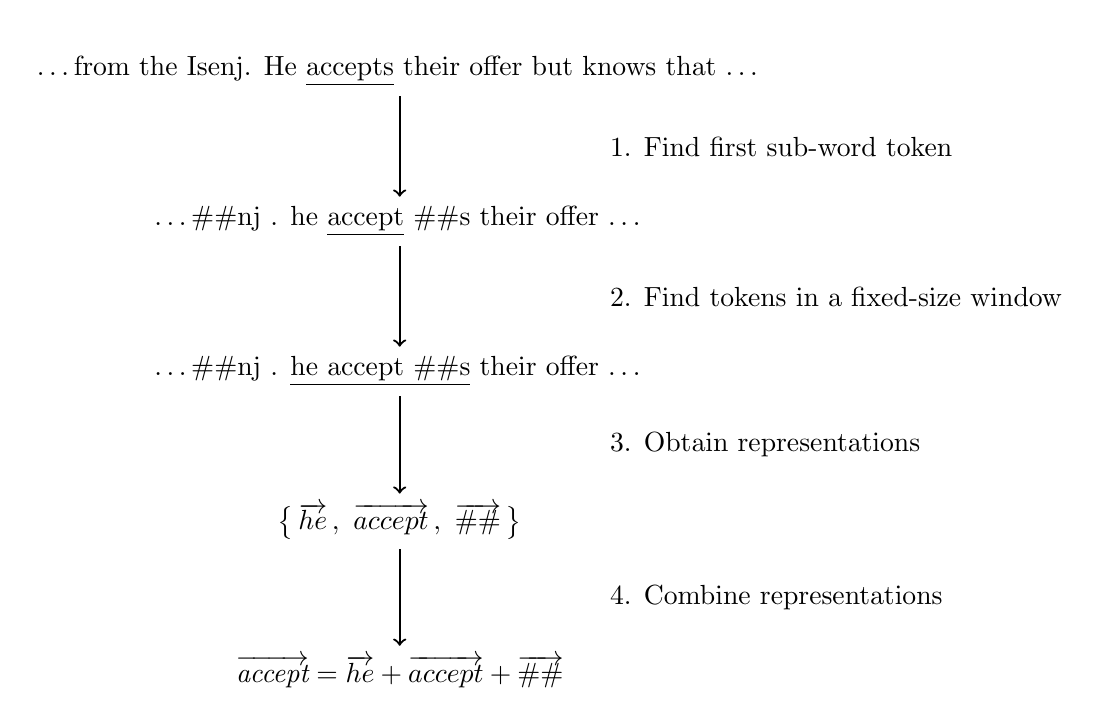
\begin{tikzpicture}[node distance=0.75in]
    \node [label] (a) {\dots from the Isenj\period{} He \underline{accepts} their offer but knows that \dots};
    \node [label, below of=a] (b) {\dots \#\#nj \period{} he \underline{accept} \#\#s their offer \dots};
    \node [label, below of=b] (c) {\dots \#\#nj \period{} \underline{he accept \#\#s} their offer \dots};
    \node [label, below of=c] (d) {$\big\{\,\ora{\text{he}}\,,\ \ora{\text{accept}}\,,\ \ora{\text{\#\#}}\,\big\}$};
    \node [label, below of=d] (e) {$\ora{\textit{accept}}=\ora{\text{he}}+\ora{\text{accept}}+\ora{\text{\#\#}}$};
    \draw [thick, ->] (a) -- (b) node[midway, right=1in] {1. Find first sub-word token};
    \draw [thick, ->] (b) -- (c) node[midway, right=1in] {2. Find tokens in a fixed-size window};
    \draw [thick, ->] (c) -- (d) node[midway, right=1in] {3. Obtain representations};
    \draw [thick, ->] (d) -- (e) node[midway, right=1in] {4. Combine representations};
  \end{tikzpicture}
  \caption{A schematic of the procedure used to obtain a contextualised representation
    of a target word from either static or contextual embeddings. In this example, the
    target word is \emph{accept}, the window size is $3$, and the composition operation
    is addition.}
\end{figure}

The basic procedure of the methods that I evaluated was as follows.
For each pair of target words and each of the two contexts in which they appear, I
obtained a contextualised representation of a target word by:
finding the index of the target word's first sub-word token within the tokens of the target word's context;
finding the tokens within a fixed-size window around the target word's first token;
obtaining the representations of the tokens in the window; and
combining the the representations to produce a single representation of the target word.

In all cases, the tokenization was performed by and the embeddings were obtained from
models available via the HuggingFace \emph{Transformers} library \parencite{Wolf2020}.
The models that I evaluated for each language are given in Table~\ref{table:language-models}.
For the static-embedding variants of the procedure, I used the models' input embeddings;
for the contextual-embedding variants, I used the models' outputs.
Several of the submissions to SemEval-2020 Task 3 used a combination of the weights of a
Transformer model's hidden states; a thorough comparison of the performance of variants
of this approach is beyond the scope of this paper.

The use of sub-word tokens means that a target word may be represented by a
different number of tokens in each context.
As a result, the representations of a pair of target words may be different in each
context, even if they are static embeddings and the window size is zero.
This explains the non-zero scores obtained by models of this kind
(Section~\ref{appendix:window-size}), most notably for the Finnish language.

\section{Results}

\subsection{Cost-benefit analysis of contextual embeddings}

\subsection{Language-specificity of window-size effects}

Generally, the scores obtained by both static- and contextual-embedding models are
maximised by a non-zero window size.
I did not perform an exhaustive search for the optimal window size due to the
computational expense.
A naïve estimation of the average number of words per context (segmenting on whitespace)
gave a result of 40-60 for the different languages, which motivated the choice of 50 as
the maximum window size to evaluate for static-embedding models.
The motivation to choose a smaller maximum window size for contextual-embedding models
was likewise economical; however, as the window size approaches the length of the
sequence, one would expect the sequence-level representation (e.g., BERT's \texttt{CLS}
token) to be a preferable choice.
These heuristics were largely confirmed by the results of the evaluation, which show
that the scores decrease as the window size approaches the maximum.

This is intuitive in the case of static embeddings, because the representations of a
target word in different contexts only differ otherwise if the target word is
represented by different sub-word tokens in each context.
In the case of contextual embeddings, a small window size is also beneficial, because
a target word may be represented by multiple sub-word tokens.
The window size that maximises the score for each language and model is given in
Table~\ref{table:best-window-size}.

\section{Conclusion}

In this paper, I have presented the results of a hypothetical submission to SemEval-2020
Task 3, ``Graded Word Similarity in Context''.
The purpose of this evaluation was to compare the performance of static and contextual
embeddings and their additive composition within a fixed-size context window on the task
of predicting the change in the human judgment of similarity of a pair of words in two
different contexts.
I found that contextual embeddings generally out-performed static embeddings, but at a
significant cost in terms of computation and memory usage; and that a small window size
improved the performance of both static and contextual embeddings, with strongly
language-specific effects.

\begin{itemize}
  \item The static embeddings of \texttt{TurkuNLP/bert-base-finnish-uncased-v1}
        outperform several of the Finnish submissions with a window size of zero.
  \item The contextual embeddings of \texttt{TurkuNLP/bert-base-finnish-uncased-v1}
        would have placed fourth and slightly improves on the baseline.
\end{itemize}
